\vspace{-1.0\baselineskip}
\section{Experiments}
\vspace{-0.4\baselineskip}
\label{sec:experiments}
We perform all experiments using our collected dataset, and evaluate multiple system settings for pose estimation and segmentation to validate each component.
For GPS and IMU signal, despite we have multiple scans for the same road segments, it is still very limited for training. Thus, follow~\cite{vishal2015accurate}, we simulate noisy GPS and IMU by adding random perturbation $\epsilon$ \wrt the ground truth pose following uniform distributions. 
%For obtaining GPS and IMU signal, due to at each round, only one sampled noisy signal can obtained. This is limited for training the system. Thus, follow~\cite{vishal2015accurate}, we simulate noisy GPS and IMU by adding random perturbation $\epsilon$ \wrt ground truth pose following uniform distributions. 
Specifically, translation and rotation noise are set as $\epsilon_t \sim U(0, 7.5m)$ and $\epsilon_r \sim U(0^{\circ}, 15^{\circ})$ respectively. 
We refer to realistic data~\cite{lee2015gps} for setting the noisy range of simulation.

\textbf{Datasets.} In this paper, our acquisition vehicle scans two sites at Beijing in China yielding two datasets. 
The first one is inside a technology park, named zhongguancun park (Zpark), and we scanned 6 rounds during different daytimes. The 3D map generated has a road length around 3$km$, and the distance between consecutive frames is around 5$m$ to 10$m$. We use 4 rounds of the video camera images for training and 2 for testing, yielding 2242 training images and 756 testing images. 
The second one we scanned 10 rounds and 4km near a lake, named daoxianghu lake (Dlake), and the distance between consecutive frames is around 1$m$ to 3$m$. 
We use 8 rounds of the video camera images for training and 2 for testing, yielding 17062 training images and 1973 testing images. 
The semantic classes of the two datasets are shown in \tabref{tbl:segment}. We will release the two datasets separately. %include $\{$sky, car-lane, pedestrian-lane, bike-lane, curb, traffic-cone, traffic-stack, traffic-fence, light-pole, traffic-light, tele-pole, traffic-sign, billboard, building, security-stand, plants, car, $\}$. 

\textbf{Implementation details.} To quickly render from the 3D map, we adopt OpenGL to efficiently render a label map with the z-buffer handling. A 512 $\times$ 608 image can be generated in 70ms with a single Titan Z GPU, which is also the input size for both pose CNN and segment CNN. 
For pose CNN, the filter sizes of all layers are $\{32, 32, 64, 128, 256, 1024, 128, 7\}$, and the forward speed for each frame is 9ms. For pose RNN, we sample sequences with length of 100 from our data for training, and the speed for each frame is 0.9ms on average.
For segment CNN, we keep the size the same as input, and the forward time is 90ms. 
Both of the network is learned with 'Nadam' optimizer~\cite{dozat2016incorporating} with a learning rate of $10^{-3}$. We sequentially train these three models due to GPU memory limitation.
Specifically, for pose CNN and segment CNN, we stops at 150 epochs when there is no performance gain, and for pose RNN, we stops at 200 epochs. For data augmentation, we use the imgaug\footnote{https://github.com/aleju/imgaug} library to add lighting, blurring and flipping variations. We keep a subset from training images for validating the trained model from each epoch, and choose the model performing best for evaluation.

For testing, since input GPS/IMU varies every time, \ie~$\ve{p}_t^c=\ve{p}^*+\epsilon$, we need to have a confidence range of prediction for both camera pose and image segment, in order to verify the improvement of each component we have is significant. Specifically, we report the standard variation of the results from a 10 time simulation to obtain the confidence range. Finally, we implement all the networks by adopting the MXNet~\cite{ChenLLLWWXXZZ15} platform.

For pose evaluation, we use the median translation offset and median relative angle~\cite{Kendall_2015_ICCV}. For evaluating segment, we adopt the commonly used pixel accuracy (Pix. Acc.), mean class accuracy (mAcc.) and mean intersect-over-union (mIOU) as that from~\cite{WuSH16e}.
% % not clear
% For testing, since input GPS/IMU contains variations, \ie $\ve{p}_t^c \sim \ve{p}^* + \epsilon$, we need to have a confidence range of prediction for both camera pose and image segmentation, in order to verify the improvement of each component we have is significant. Specifically, we report the standard variation of the results from a 10 time simulation to obtain the confidence range. Finally, we implement all the networks by adopting the MXNet~\cite{ChenLLLWWXXZZ15} platform.

% \textbf{Pose Evaluation.}
% In \tabref{tbl:pose}, we show the performance of estimated translation $\ve{t}$ and rotation $\ve{r}$ from different model variations. We first directly follow the work of PoseNet~\cite{Kendall_2015_ICCV,kendall2017geometric}, and use their published code and geometric loss (\equref{eq:proj_loss}) to train a model. 
% Due to scene appearance similarity of the street-view, we did not obtain a reasonable model, \ie results better than the noisy GPS/IMU signal.
% At the 2nd row, we show the median error of GPS and IMU from our simulation. At the 3rd row, by using our pose CNN, the model can learn good relative pose from camera and GPS/IMU, which significantly reduces the error (60$\%$ for $\ve{t}$, 85$\%$ for $\ve{r})$. 
% By adding semantic cues, \ie road priori and semantic weights in \equref{eq:proj_loss}, the pose errors are further reduced, especially for rotation (from $0.982$ to $0.727$ at the 4th row). 

% When experiments with an online video, we setup a baseline of performing RNN directly on the GPS/IMU signal, and as shown at 'Pose RNN w/o CNN', the estimated $\ve{t}$ is even better than pose CNN, while $\ve{r}$ is comparably much worse. This meets our expectation since the speed of camera is easier to capture temporally than rotation. Another baseline we adopt is performing Kalman filter~\cite{kalman1960new} to the output from Pose CNN by assuming a constant speed which we set as the averaged speed from training sequences. As shown at 'Pose CNN w KF', it does improve slightly for translation, but harms rotation, which means the filter over smoothed the sequence. Finally when combining pose CNN and RNN, it achieves the best pose estimation both for $\ve{t}$ and $\ve{r}$.

% % Finally, RNN gives strong cues about the moving speed and acceleration of the camera, yields the best results for both translation and rotation.
% >>>>>>> e803c32c4f5e73341b05602b6a5ced7c121830f3
\begin{table}
\vspace{-0\baselineskip}
\center
\fontsize{6.5}{7}\selectfont
\hspace*{-0.23cm}
\begin{tabular}{lllll}
\toprule[0.1 em]
% \thickhline
%& PoseNet~\cite{kendall2017geometric} & -  & -  & -  \\
Data & Method & Trans (m) $\downarrow$ & Rot ($\circ$)$\downarrow$  & Pix. Acc($\%$)$\uparrow$ \\
\hline
\parbox[t]{2mm}{\multirow{6}{*}{\rotatebox[origin=c]{90}{Zpark}}} & Noisy pose & 3.45 $\pm$ 0.176 & 7.87 $\pm$ 1.10 & 54.01 $\pm$ 1.5 \\
& Pose CNN w/o semantic & 1.355 $\pm$ 0.052  & 0.982 $\pm$ 0.023 & 70.99 $\pm$ 0.18 \\
& Pose CNN w semantic & 1.331 $\pm$ 0.057  & 0.727 $\pm$ 0.018 & 71.73 $\pm$ 0.18  \\
& Pose RNN w/o CNN & 1.282 $\pm$ 0.061  & 1.731 $\pm$ 0.06 &  68.10 $\pm$ 0.32 \\
& Pose CNN w KF & 1.281 $\pm$ 0.06  & 0.833 $\pm$ 0.03 & 72.00 $\pm$ 0.17  \\
& Pose CNN-RNN  & \textbf{1.005} $\pm$ 0.044  & \textbf{0.719} $\pm$ 0.035  & \textbf{73.01} $\pm$ 0.16  \\
\toprule[0.1 em]
\hline
\parbox[t]{1mm}{\multirow{3}{*}{\rotatebox[origin=c]{90}{Dlake}}} & Pose CNN w semantic & 1.667 $\pm$ 0.05 & 0.702 $\pm$ 0.015 & 87.83 $\pm$ 0.017 \\
& Pose RNN w/o CNN & 1.385 $\pm$ 0.057 & 1.222 $\pm$ 0.054 & 85.10 $\pm$ 0.03\\
& Pose CNN-RNN  & \textbf{0.890} $\pm$ 0.037  & \textbf{0.557}$\pm$ 0.021 & \textbf{88.55} $\pm$ 0.13  \\
\toprule[0.1 em]
\end{tabular}
\caption{Compare the accuracy of different settings for pose estimation from the two datasets.
Noisy pose indicates the noisy input signal from GPS, IMU, and 'KF' means kalman filter.
The number after $\pm$ indicates the standard deviation (S.D.) from 10 simulations. $\downarrow \& \uparrow$ means lower the better and higher the better respectively. 
We can see the improvement is statistically significant.}
\label{tbl:pose}
\vspace{-2.5\baselineskip}
\end{table}

\textbf{Pose Evaluation.}
In \tabref{tbl:pose}, we show the performance of estimated translation $\ve{t}$ and rotation $\ve{r}$ from different model variations. 
We first directly follow the work of PoseNet~\cite{Kendall_2015_ICCV,kendall2017geometric}, and use their published code and geometric loss (\equref{eq:proj_loss}) to train a model on Zpark dataset. 
Due to scene appearance similarity of the street-view, we did not obtain a reasonable model, \ie~results better than the noisy GPS/IMU signal.
At the 1st row, we show the median error of GPS and IMU from our simulation. 
At the 2nd row, by using our pose CNN, the model can learn good relative pose between camera and GPS/IMU, which significantly reduces the error (60$\%$ for $\ve{t}$, 85$\%$ for $\ve{r})$. 
By adding semantic cues, \ie road priori and semantic weights in \equref{eq:proj_loss}, the pose errors are further reduced, especially for rotation (from $0.982$ to $0.727$ at the 3rd row). In fact, we found the most improvement is from semantic weighting, while the road priori helps marginally. In our future work, we would like to experiment larger noise and more data variations, which will better validate different cues.

For evaluating an video input, we setup a baseline of performing RNN directly on the GPS/IMU signal, and as shown at 'Pose RNN w/o CNN', the estimated $\ve{t}$ is even better than pose CNN, while $\ve{r}$ is comparably much worse. This meets our expectation since the speed of camera is easier to capture temporally than rotation. Another baseline we adopt is performing Kalman filter~\cite{kalman1960new} to the output from Pose CNN by assuming a constant speed which we set as the averaged speed from training sequences. As shown at 'Pose CNN w KF', it does improve slightly for translation, but harms rotation, which means the filter over smoothed the sequence. Finally when combining pose CNN and RNN, it achieves the best pose estimation both for $\ve{t}$ and $\ve{r}$. We visualize some results at \figref{fig:results}(a-c).
Finally at bottom of \tabref{tbl:pose}, we list corresponding results on Dlake dataset, which draws similar conclusion with that from Zpark dataset.

% Finally, RNN gives strong cues about the moving speed and acceleration of the camera, yields the best results for both translation and rotation.

\begin{table*}[t]
\center
\vspace{-0.5\baselineskip}
\fontsize{6.5}{7}\selectfont
\setlength\tabcolsep{1.5pt}
% \begin{tabular}{lccccccccccccccccccccc}
% \toprule[0.1 em]
%\thickhline
% Method & \rot{mIOU} & \rot{mAcc} & \rot{Pix. Acc}   & \rot{sky} & \rot{car-lane} & \rot{ped-lane} & \rot{bike-lane} & \rot{curb} & \rot{$t$-cone} & \rot{$t$-stack} & \rot{$t$-fence} & \rot{light-pole} & \rot{$t$-light} & \rot{tele-pole} & \rot{$t$-sign} & \rot{billboard} & \rot{temp-build} & \rot{building} & \rot{sec.-stand} & \rot{plants} & \rot{object} \\
% \hline
% ResNet38~\cite{WuSH16e}                      &64.66  &71.92 & 95.87 &93.6 &98.5 &82.9 &87.2 &61.8 &46.1 &41.7 &82.0 &37.5 &26.7 &45.9 &49.5 &60.0 &85.1 &67.3 &38.0 &89.2 &66.3\\
% Render PoseRNN                               &32.61  & -    &91.7 &50.4 &62.1 &16.9 &6.6 &5.8 &30.5 &8.9 &6.7 &10.1 &16.3 &22.2 &70.6 &29.4 &20.2 &73.5 & - \\
% SegCNN w/o Pose                              &68.35  &77.09 & 95.61 &94.2 &98.6 &83.8 &89.5 &69.3 &47.5 &52.9 &83.9 &52.2 &43.5 &46.3 &52.9 &66.9 &87.0 &69.2 &40.0 &88.6 &63.8 \\
% SegCNN w pose GT                             &79.37  &86.8  & 97.1  &96.1 &99.4 &92.5 &93.9 &81.4 &68.8 &71.4 &90.8 &71.7 &64.2 &69.1 &72.2 &83.7 &91.3 &76.2 &58.9 &91.6 &56.7 \\
% %SegCNN w Pose CNN &68.6$\pm$0.12 & 77.95$\pm$0.16 & 95.67$\pm$0.01  &94.5 &98.7 &84.3 &89.3 &69.0 &46.8 &52.9 &84.9 &53.7 &39.5 &48.8 &50.4 &67.9 &87.5 &69.9 &42.8 &88.5 &60.9 \\
% SegCNN w Pose CNN &68.6 & 77.95$\pm$0.16 & 95.67$\pm$0.01  &94.5 &98.7 &84.3 &89.3 &69.0 &46.8 &52.9 &84.9 &53.7 &39.5 &48.8 &50.4 &67.9 &87.5 &69.9 &42.8 &88.5 &60.9 \\
% SegCNN Final    &\textbf{69.93}$\pm$0.08  & \textbf{79.36}$\pm$0.08 &\textbf{95.98}$\pm$0.004 &
%                                              94.9 &98.8 &85.3 &90.2 &71.9 &45.7 &57.0 &85.9 &58.5 &41.8 &51.0 &52.2 &69.4 &88.5 &70.9 &48.0 &89.3 &59.5 \\
% \toprule[0.1 em]
% \vspace{-2.0\baselineskip}
% \end{tabular}
\begin{tabular}{llcccccccccccccccccccc}
\vspace{-1.0\baselineskip}
% \toprule[0.1 em]
%\thickhline
Data & \multicolumn{1}{c}{Method} & \rot{mIOU}  & \rot{Pix. Acc}   & \rot{sky} & \rot{car-lane} & \rot{ped-lane} & \rot{bike-lane} & \rot{curb} & \rot{$t$-cone} & \rot{$t$-stack} & \rot{$t$-fence} & \rot{light-pole} & \rot{$t$-light} & \rot{tele-pole} & \rot{$t$-sign} & \rot{billboard} & \rot{temp-build} & \rot{building} & \rot{sec.-stand} & \rot{plants} & \rot{object} \\
\hline
\parbox[t]{2mm}{\multirow{6}{*}{\rotatebox[origin=c]{90}{Zpark}}} & 
ResNet38~\cite{WuSH16e}     &64.66   & 95.87 &93.6 &98.5 &82.9 &87.2 &61.8 &46.1 &41.7 &82.0 &37.5 &26.7 &45.9 &49.5 &60.0 &85.1 &67.3 &38.0 &89.2 &66.3\\
&Render PoseRNN              &32.61  & 73.1 & - & 91.7 &50.4 &62.1 &16.9 &6.6 &5.8 &30.5 &8.9 &6.7 &10.1 &16.3 &22.2 &70.6 &29.4 &20.2 &73.5 & - \\
&SegCNN w/o Pose             &68.35   & 95.61 &94.2 &98.6 &83.8 &89.5 &69.3 &47.5 &52.9 &83.9 &52.2 &43.5 &46.3 &52.9 &66.9 &87.0 &69.2 &40.0 &88.6 &63.8 \\
&SegCNN w pose GT            &79.37   & 97.1  &96.1 &99.4 &92.5 &93.9 &81.4 &68.8 &71.4 &90.8 &71.7 &64.2 &69.1 &72.2 &83.7 &91.3 &76.2 &58.9 &91.6 &56.7 \\
&SegCNN w Pose CNN           &68.6  & 95.67  &94.5 &98.7 &84.3 &89.3 &69.0 &46.8 &52.9 &84.9 &53.7 &39.5 &48.8 &50.4 &67.9 &87.5 &69.9 &42.8 &88.5 &60.9 \\
&SegCNN w Pose RNN &\textbf{69.93}  &\textbf{95.98} &
                                             94.9 &98.8 &85.3 &90.2 &71.9 &45.7 &57.0 &85.9 &58.5 &41.8 &51.0 &52.2 &69.4 &88.5 &70.9 &48.0 &89.3 &59.5 \\
\toprule[0.1 em]
\end{tabular}
\vspace{-0.8\baselineskip}
\begin{tabular}{llcccccccccccccccccccccc}
\vspace{-2.0\baselineskip}
Data& \multicolumn{1}{c}{Method} & \rotf{mIOU} & \rotf{Pix. Acc}  & \rotf{sky} & \rotf{car-lane} & \rotf{ped-lane}  & \rotf{$t$-stack} & \rotf{$t$-fence} & \rotf{wall} & \rotf{light-pole} & \rotf{$t$-light} & \rotf{tele-pole} & \rotf{$t$-sign} & \rotf{billboard} & \rotf{building} & \rotf{plants} & \rotf{car} & \rotf{cyclist} & \rotf{motorbike} & \rotf{truck} & \rotf{bus}\\
\hline
\parbox[t]{2mm}{\multirow{3}{*}{\rotatebox[origin=c]{90}{Dlake}}} & 
SegCNN w/o Pose  &62.36 &96.7 &95.3 &96.8 &12.8 &21.5 &81.9 &53.0 &44.7 &65.8 &52.1 &87.2 &55.5 &66.8 &94.5 &84.9 &20.3 &28.9 &78.4 &82.1 \\
&SegCNN w pose GT &73.10 &97.7 &96.8 &97.5 &41.3 &54.6 &87.5 &70.5 &63.4 &77.6 &70.5 &92.1 &69.2 &77.4 &96.1 &87.4 &24.5 &43.8 &80.0 &85.7 \\
&SegCNN w pose RNN &\textbf{67.00} &\textbf{97.1} &95.8 &97.2 &30.0 &37.4 &84.2 &62.6 &47.4 &65.5 &62.9 &89.6 &59.0 &70.3 &95.2 &86.8 &23.9 &34.4 &76.8 &86.6 \\
\toprule[0.1 em]
\end{tabular}
\caption{Compare the accuracy of different segment networks setting over Zpark (top) and Dlake (bottom) dataset. $t$ is short for 'traffic' in the table. Here we drop the 10 times S.D. to save space because it is relatively small. Our results are especially good at parsing of detailed structures and scene layouts, which is visualized in~\figref{fig:results}.}
\label{tbl:segment}
\vspace{-1.2\baselineskip}
\end{table*}


\begin{figure*}[!htbp]
\center
\vspace{-0.3\baselineskip}
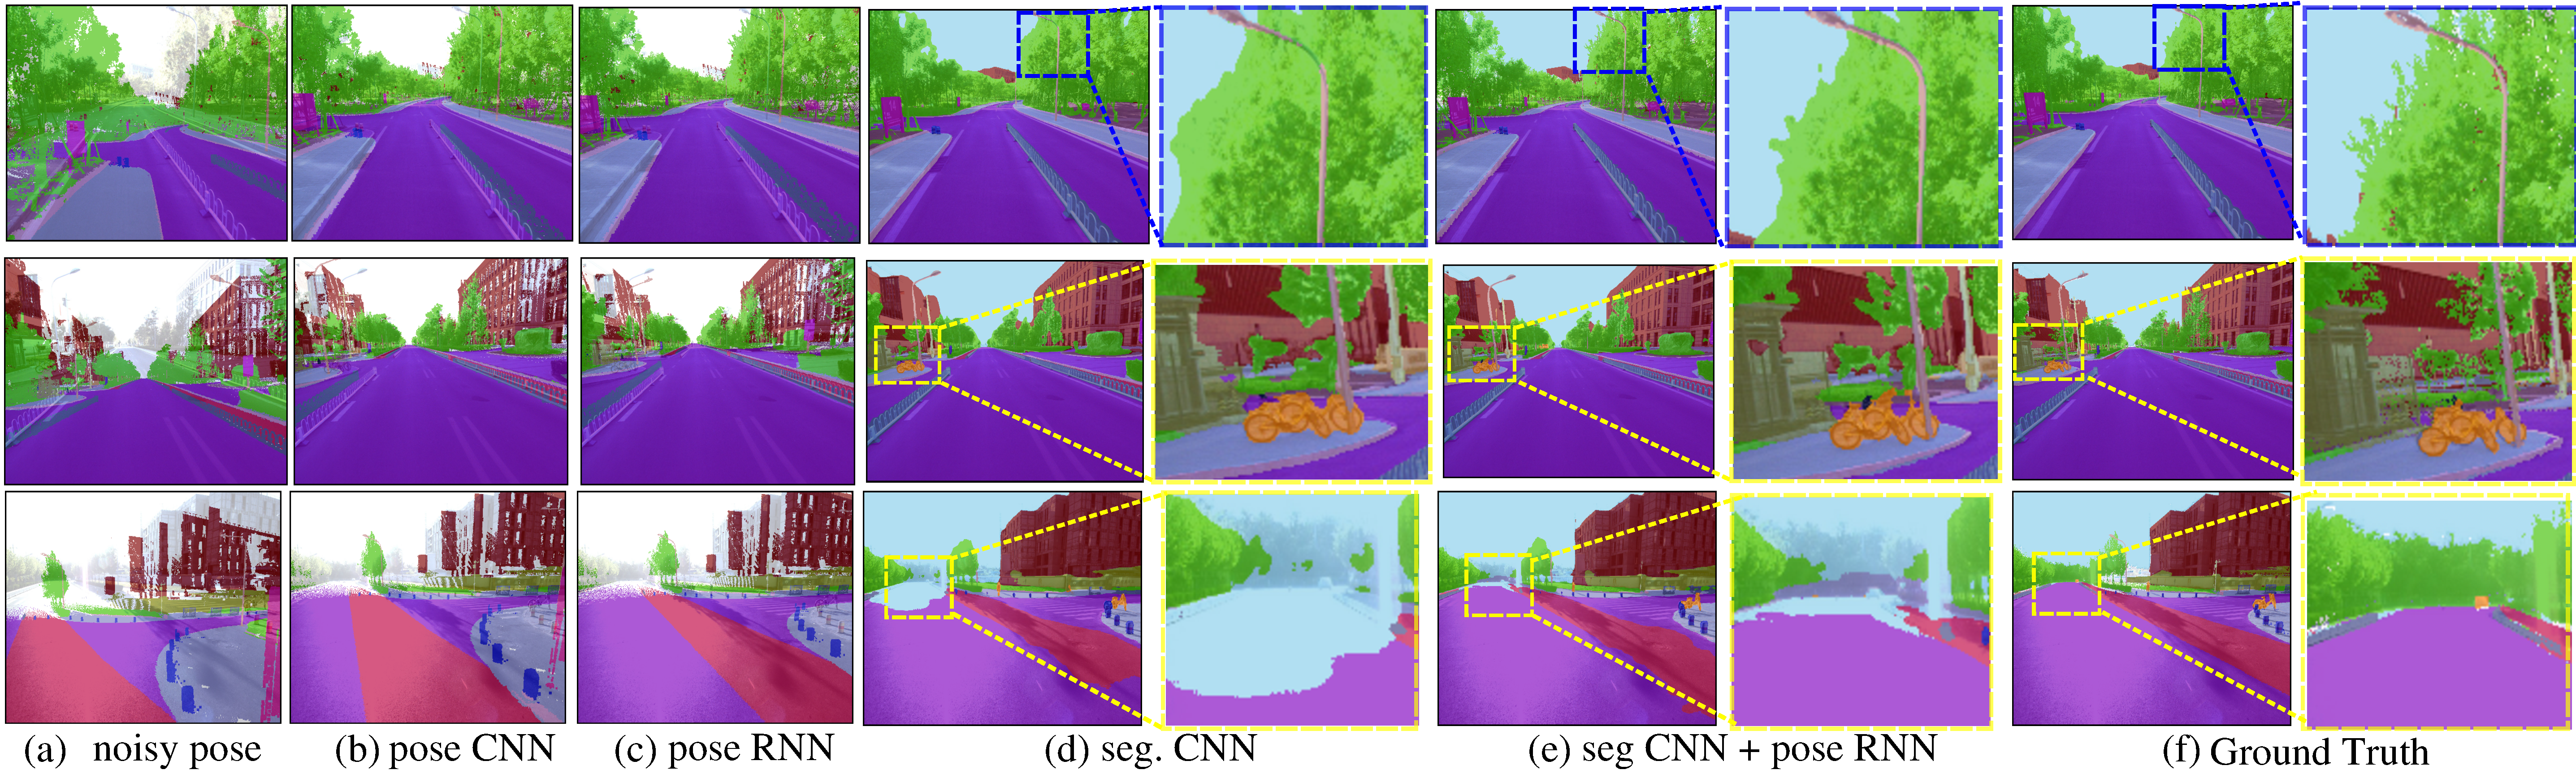
\includegraphics[width=0.99\textwidth]{fig/results_v2.png}
   \caption{Results from each intermediate stage out of the system over Zpark dataset. Label map is overlaid with the image. Improved regions are boxed and zoomed out (best in color). More results are available in the supplementary material.}
\label{fig:results}
\vspace{-1.2\baselineskip}
\end{figure*}
\textbf{Segment Evaluation.}
At top part of \tabref{tbl:segment}, we show the scene parsing results of Zpark dataset. 
Firstly, we adopt one of the SOTA parsing network on the CityScapes, \ie~ResNet38~\cite{WuSH16e}, and train it with Zpark dataset. It utilizes pre-trained parameters from the CityScapes~\cite{Cordts2016Cityscapes} dataset, and run with a 1.03$s$ per-frame with our resolution. 
As shown at the 1st row, it achieve reasonable accuracy compare to our segment CNN (2nd row) when there is no pose priori. However, our network is 10x faster. 
At 3rd row, we show the results of rendered label map with the estimated pose from pose RNN. Clearly, the results are much worse due to missing pixels and object misalignment.
At 4th row, we use the rendered label map with ground truth pose as segment CNN guidance to obtain an upper-bound for our segmentation performance. 
In this case, the rendered label map aligns perfectly with the image, thus significantly improves the results by correct labelling most of the static background.
% At 4th row, we train the segment network without pose prior.  
At 5th and 6th row, we show the results trained with rendered label map with pose after pose CNN and pose RNN respectively. We can see using pose CNN, the results just improve slightly compare to the segment CNN. From our observation, this is because the offset is still significant for some detailed structures, \eg light-pole.
% Notice that for a fair comparison, after convergence of segment CNN, we continue training the network another 100 epochs in order to avoid the influence from longer training.

% =======
% Firstly, we adopt one of the SOTA parsing network on the CityScapes, \ie ResNet38~\cite{WuSH16e}, and train it with our data. It has pre-trained parameters from the ImageNet~\cite{deng2009imagenet} dataset, and run with a 1.03$s$ per-frame with our resolution. As shown at the 1st row, it achieve reasonable accuracy compare to our segment CNN (2nd row) when there is no pose priori. 
% However, our network is 10x faster, and runs in 90ms. 
% At the 3rd row, we use the rendered label map with the ground truth pose as segment CNN priori to obtain an upper-bound for the segmentation performance.
% In this case, the rendered label map aligns perfect with the image, thus yields significantly better results without miss classify most of the static background.
% % At 4th row, we train the segment network without pose prior.  
% % Notice that for a fair comparison, after convergence at 100 epoch, we continue train the network another 100 epochs in order to avoid the influence from longer training.
% At the 4th and 5th row, we show the results trained with rendered label map with the pose from pose CNN and pose CNN-RNN respectively. We can see using pose CNN, the results just improve slightly compare to the segment CNN, from our observation, this is because the offset between rare classes is still significant.
% >>>>>>> e803c32c4f5e73341b05602b6a5ced7c121830f3
However, when using the pose after RNN, better alignment is achieved, and the segment accuracy is improved significantly especially for thin structured regions like pole, as visualized in~\figref{fig:results}, which demonstrates the effectiveness of our strategy. We list the results over Dlake dataset with more object labelling at bottom part of \tabref{tbl:segment}, and here the rendered label provides a background context for object segmentation, which also improve the object parsing performance. 
% Here, we leave per-class results to the supplementary materials as space limitation.

% \begin{table}[b]
% \vspace{-1.0\baselineskip}
% \center
% \hspace*{-0.3cm}
% \fontsize{8}{8}\selectfont
% \begin{tabular}{lccc}
% \toprule[0.1 em]
% %\thickhline
% Method & mIOU($\%$) $\uparrow$ &  mAcc($\%$) $\uparrow$& Pix. Acc($\%$) $\uparrow$ \\
% \hline
% ResNet38~\cite{WuSH16e} &64.66  & 71.92 & 95.87  \\
% SegCNN w/o Pose & 68.35 & 77.09 & 95.61 \\
% SegCNN w pose GT &79.37  & 86.8 & 97.1 \\
% % SegCNN $\xi$ Pose & 95.63 $\pm$ 0.02 & 77.39 $\pm$ 0.21 & 68.41 $\pm$ 0.15\\
% SegCNN w Pose CNN &68.6 $\pm$ 0.12 & 77.95 $\pm$ 0.16 & 95.67 $\pm$ 0.01 \\
% SegCNN Final & \textbf{69.93} $\pm$ 0.08  & \textbf{79.36} $\pm$ 0.08 &\textbf{95.98} $\pm$ 0.004 \\
% \toprule[0.1 em]
% \end{tabular}
% \caption{Compare the accuracy of different network settings. $\pm$ indicates the standard variation by 10 times GPS simulation. 
% Full table for all class accuracy is available in our supplementary materials.}
% \label{tbl:segment}
% <<<<<<< HEAD
% \vspace{-1.3\baselineskip}
% \end{table}

In \figref{fig:results}, we visualize several examples from our results at the view of camera. In the figure, we can see the noisy pose (a), is progressively rectified by pose CNN (b) and pose RNN (c) from view of camera. 
Additionally, at (d) and (e), we compare the segment results without and with camera pose respectively. As can be seen at the boxed regions, the segment results with rendered label maps provide better accuracy in terms of capturing region details at the boundary, discovering rare classes and keeping correct scene layout. All of above could be important for applications, \eg figuring out the traffic signs and tele-poles that are visually hard to detect.
% =======
% \vspace{-0.3\baselineskip}
% \end{table*}

% \begin{table}
% \center
% \fontsize{8}{9}\selectfont
% \begin{tabular}{lccc}
% \toprule[0.1 em]
% %\thickhline
% Method &Pix. Acc ($\%$) &  mAcc ($\%$) & mIOU ($\%$) \\
% \hline
% ResNet38~\cite{WuSH16e} & 95.87 & 71.92 & 64.66 \\
% SegCNN w/o Pose & 95.61 & 77.09 & 68.35 \\
% SegCNN w Pose GT & 97.1 & 86.8 & 79.37 \\
% % SegCNN $\xi$ Pose & 95.63 $\pm$ 0.02 & 77.39 $\pm$ 0.21 & 68.41 $\pm$ 0.15\\
% SegCNN w Pose CNN & 95.67 $\pm$ 0.01 & 77.95 $\pm$ 0.16 & 68.6 $\pm$ 0.12\\
% SegCNN Final & \textbf{95.98} $\pm$ 0.004 & \textbf{79.36} $\pm$ 0.08 & \textbf{69.93} $\pm$ 0.08 \\
% \toprule[0.1 em]
% \end{tabular}
% \caption{Compare the accuracy of different network settings. $\pm$ indicates the standard variation by 10 times GPS simulation. 
% The meaning of each label map for an image is indicated by a layout map at left top. Improved regions are boxed and zoomed out for better visualization.
% Full table for all class accuracy is available in our supplementary materials.}
% \label{tbl:segment}
% \vspace{-0.3\baselineskip}
% \end{table}

% In \figref{fig:results}, we visualize several examples from our dataset. In the figure, we can see the noisy pose (b), is progressively rectified by pose CNN (c) and pose RNN (d) \wrt the camera image. Additionally, at (e) and (f), we compare the segmentation results without and with camera pose respectively. As can be seen at the boxed regions, the segmentation results with pose rendered label maps do provide better accuracy, in terms of capturing detailed regions and rare classes.
% >>>>>>> e803c32c4f5e73341b05602b6a5ced7c121830f3
